\setcounter{ExampleCounter}{1}
As we saw with the last few examples in the previous section, linear models often break down over the long term; in fact, few natural phenomena actually follow linear trends, so at best linear models are usually just a rough short-term approximation.  On the other hand, many applications follow \textbf{exponential growth.}  One of the most common is population growth, so we'll use an example of that for illustration.

Suppose you're tracking the population of fish in a lake, and every year 10\% of the fish have surviving offspring.  Notice that this is still a simplified model, since more sophisticated models account for predators, limited resources, and so on.  In our simple model, though, an initial population of 1000 fish would grow to 1100 fish after the first year, and each subsequent year, 10\% of the population at that time will be added, so the population grows faster as it gets larger.

The recursive model is shown below.
\begin{align*}
P_0 &= 1000\\
P_t &= P_{t-1} + 0.10P_{t-1}
\end{align*}

We can use this to derive a closed-form model:
\begin{align*}
P_0 &= 1000\\
P_1 &= P_0 + 0.10P_0 = P_0(1+0.10) = P_0 \cdot 1.10\\
P_2 &= P_1 \cdot 1.10 = P_0 \cdot 1.10 \cdot 1.10 = P_0 \cdot 1.10^2\\
P_3 &= P_2 \cdot 1.10 = P_0 \cdot 1.10^3\\
&\vdots\\
P_t &= P_0 \cdot 1.10^t
\end{align*}

The \textbf{growth rate} is 10\%, and 1.10 is the \textbf{growth multiplier}.  Each year's population is 1.10 times the previous year's population.

\begin{center}
\begin{tabular}{c | c | c}
\textbf{Year} & \textbf{Population} & \textbf{Growth from Previous Year}\\
\hline
0 & 1000 &\\
1 & 1100 & 100\\
2 & 1210 & 110\\
3 & 1331 & 121\\
4 & 1464 & 133\\
5 & 1611 & 147\\
6 & 1772 & 161
\end{tabular}
\end{center}
Notice that there is a constant \textit{percentage} growth, so as the population increases, the number by which it grows gets larger each year.\\

If we plot these first few values, the graph is not quite linear, but it's not that far from a linear plot.  Because of this, in the short term, linear models can approximate exponential models, even if it isn't a perfect fit.
\begin{center}
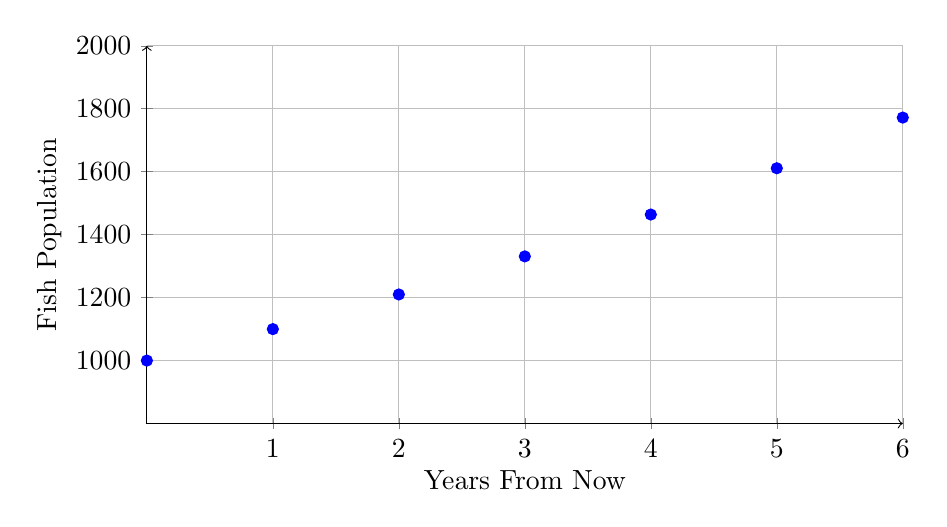
\begin{tikzpicture}
\begin{axis}[
    xmin=0, xmax=6,
    ymin=800, ymax=2000,
    axis lines=center,
    axis on top=false,
    domain=0:1,
    x=1.6cm,
    y=0.004cm,
    xtick={0,1,...,6},
    xticklabels={0,1,...,6},
    ytick={0,200,...,2000},
    yticklabels={0,200,...,2000},
    axis lines=middle,
    axis line style={->},
    x label style={at={(axis description cs:0.5,-0.1)},anchor=north},
    y label style={at={(axis description cs:-0.1,.5)},rotate=90,anchor=south},
    xlabel={Years From Now},
    ylabel={Fish Population},
    grid=major
    ]
	\addplot [blue,only marks] table {
	0 1000
	1 1100
	2 1210
	3 1331
	4 1464
	5 1611
	6 1772
	};
\end{axis}
\end{tikzpicture}
\end{center}
%\begin{center}
%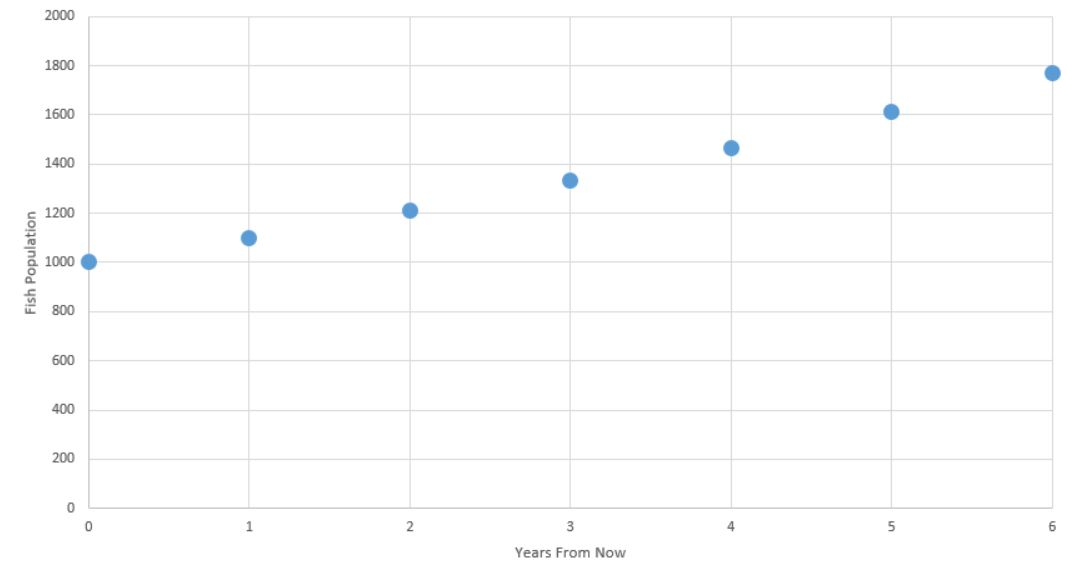
\includegraphics[width=0.7\textwidth]{ExpGrowthLinear}
%\end{center}
\vfill
\pagebreak

As we begin to project further into the future, though, the model clearly deviates from a linear trend:
\begin{center}
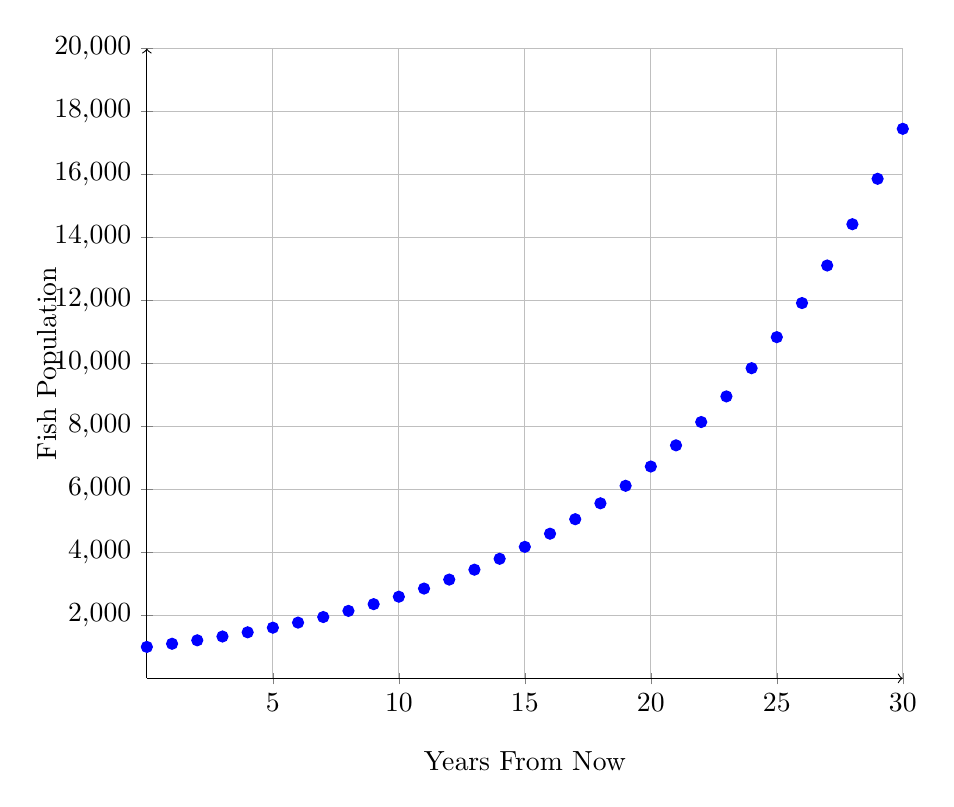
\begin{tikzpicture}
\begin{axis}[
    xmin=0, xmax=30,
    ymin=0, ymax=20,
    axis lines=center,
    axis on top=false,
    domain=0:1,
    x=0.32cm,
    y=0.4cm,
    xtick={0,5,...,30},
    xticklabels={0,5,...,30},
    ytick={0,2,...,20},
    yticklabels={0,{2,000},{4,000},{6,000},{8,000},{10,000},{12,000},{14,000},{16,000},{18,000},{20,000}},
    axis lines=middle,
    axis line style={->},
    x label style={at={(axis description cs:0.5,-0.1)},anchor=north},
    y label style={at={(axis description cs:-0.1,.5)},rotate=90,anchor=south},
    xlabel={Years From Now},
    ylabel={Fish Population},
    grid=major
    ]
	\addplot [blue,only marks] table {
	0 1
	1 1.1
	2 1.21
	3 1.331
	4 1.464
	5 1.611
	6 1.772
	7 1.949
	8 2.144
	9 2.358
	10 2.594
	11 2.853
	12 3.138
	13 3.452
	14 3.798
	15 4.177
	16 4.595
	17 5.055
	18 5.56
	19 6.116
	20 6.728
	21 7.4
	22 8.14
	23 8.954
	24 9.85
	25 10.835
	26 11.918
	27 13.11
	28 14.421
	29 15.863
	30 17.45
	};
\end{axis}
\end{tikzpicture}
\end{center}
%\begin{center}
%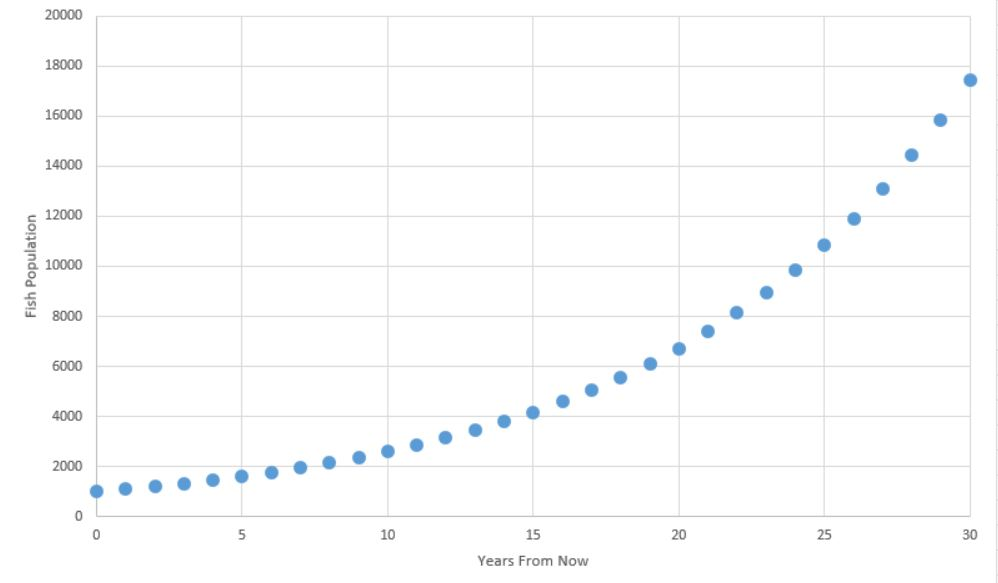
\includegraphics[width=0.7\textwidth]{ExpGrowthExponential}
%\end{center}

If the population had been growing linearly by 100 fish each year, the population at the end of 30 years would have only been 4000 instead of nearly 18,000 under the exponential model.  Most of this growth occurred in the second half; this is typical of exponential growth.  Since the growth from one year to another depends on the size of the population, it grows much faster near the end, and the growth begins to snowball.

\begin{formula}{Exponential Growth}
If a quantity starts at size $P_0$ and grows by $R\%$ (written as a decimal, $r$) every time period, then the quantity after $t$ time periods is given by
\[P_t = P_0 (1+r)^t\]
The \textbf{growth rate} is $r$, and the \textbf{growth multiplier} is $1+r$.

If $r$ is negative, then instead of exponential growth there is \textbf{exponential decay}.
\end{formula}

The growth multiplier is the common ratio between terms, and it can be used to recognize exponential growth from data, just like a common difference between terms can be used to recognize linear growth.
\begin{center}
\begin{tabular}{c | c | c}
\textbf{Year} & \textbf{Population} & \textbf{Ratio to Previous Year}\\
\hline
0 & 1000 &\\
1 & 1100 & 1.1\\
2 & 1210 & 1.1\\
3 & 1331 & 1.1\\
4 & 1464 & 1.1\\
5 & 1611 & 1.1\\
6 & 1772 & 1.1
\end{tabular}
\end{center}
\pagebreak

\begin{example}[https://www.youtube.com/watch?v=NHLi7ekPSPM]{Frederick Population}
The population of Frederick County grew from 239,520 in 2012 to 241,409 in 2013, a growth of about 0.8\%.  If this growth rate continues, what is the population of Frederick County expected to be in 2025?\\

\marginnote{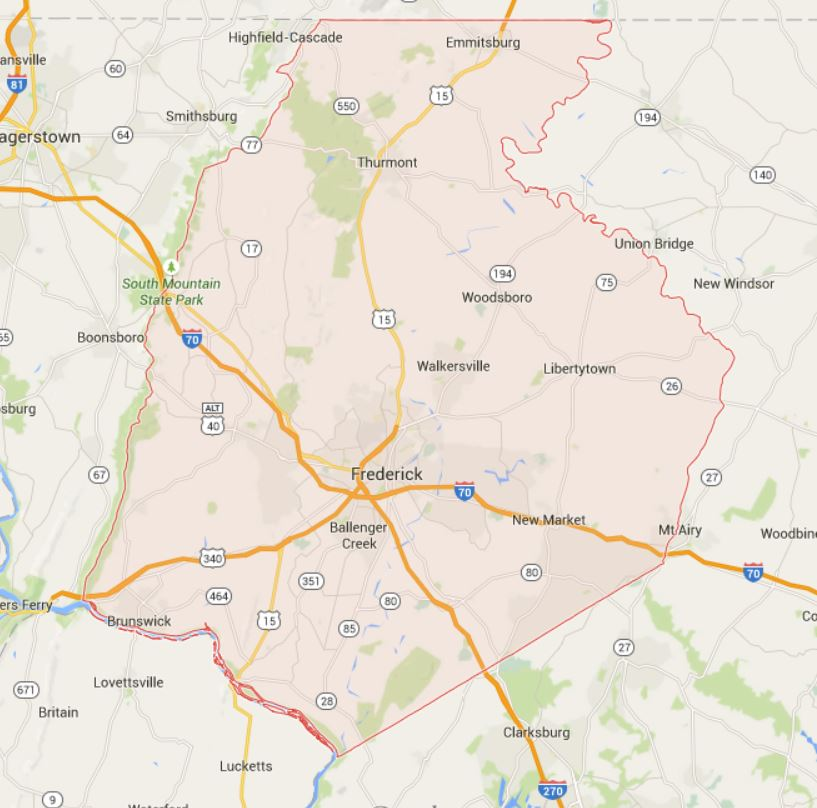
\includegraphics[scale=0.15]{FrederickCountyMap1}}
If $r=0.008$, we can use the exponential growth formula to predict the population in 2025.  To do so, however, we need to pick a year to be year 0.  Since we're given the population in 2012 and 2013, we can use either one, but we'll choose 2013, so 2025 will be year 12.
\begin{align*}
P_{12} &= P_0 (1+r)^t\\
&= 241,409(1+0.008)^{12}\\
&= 265,632
\end{align*}
We expect the population of Frederick County to reach 265,632 by 2025.
\end{example}

\begin{try}[http://www.izzomath.com/103text/growthmodels/example2.1/story.html]
\begin{tabular}{b{2in} c}
India is the second most populous country in the world, with a population of about 1.252 billion in 2013.  The population is growing by about 1.21\% each year.

If this trend continues, what is India's population expected to grow to by 2030? & 
\includegraphics[width=0.5\textwidth]{IndiaMap1}
\end{tabular}
\end{try}

\begin{proc}{Using Your Calculator: Exponents}
\begin{tabular}{c l}
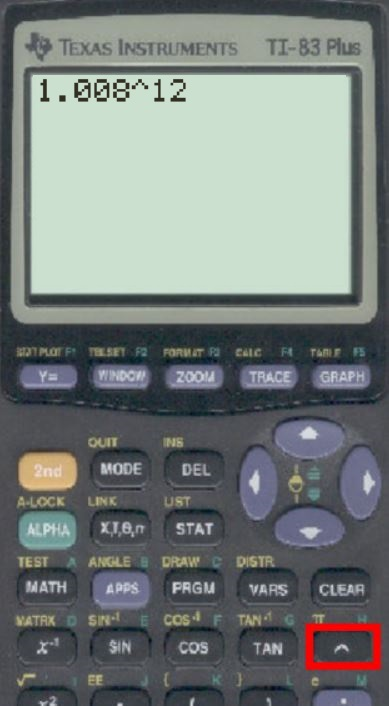
\includegraphics[scale=0.35]{Calculator2} & \parbox[b]{3in}{To evaluate expressions like $1.008^{12}$, we'll use the exponent function on a calculator rather than multiplying 1.008 by itself 12 times.  The exponent function is usually labeled like one of the following:
\begin{center}
\begin{tabular}{c c c}
$\boxed{\wedge}$ & $\boxed{y^x}$ & $\boxed{x^y}$
\end{tabular}
\end{center}

To evaluate $1.008^{12}$, we'd type $1.008 \ \boxed{\wedge}\ 12$ or $1.008\ \boxed{y^x}\ 12$.  Try it and make sure that you get an answer around 1.100338694.}
\end{tabular}
\end{proc}
\pagebreak

\begin{example}[https://www.youtube.com/watch?v=_u9RlZX_BkI]{Tuition Prediction}
A friend is using the equation \[P_t = 4600(1.072)^t\] to predict the annual tuition at a local college.  She says that the formula is based on years after 2010.  What does this equation tell us?\\

\marginnote{\bfseries Solution}
In this equation, $P_0 = 4600$, which is the initial tuition, so we infer that the tuition in 2010 is \$4600.

The growth multiplier is 1.072, so the growth rate is 0.072 or 7.2\%.  We expect tuition to grow by 7.2\% each year.
\end{example}

\begin{example}[https://www.youtube.com/watch?v=2wtJ_T3_e7o]{Carbon Dioxide Emissions}
In 1990, the residential energy use in the US was responsible for 962 million metric tons of carbon dioxide emissions.  By the year 2000, that number had risen to 1182 million metric tons.  If the emissions grow exponentially and continue at the same rate, what will the emissions grow to by 2050?\\

\marginnote{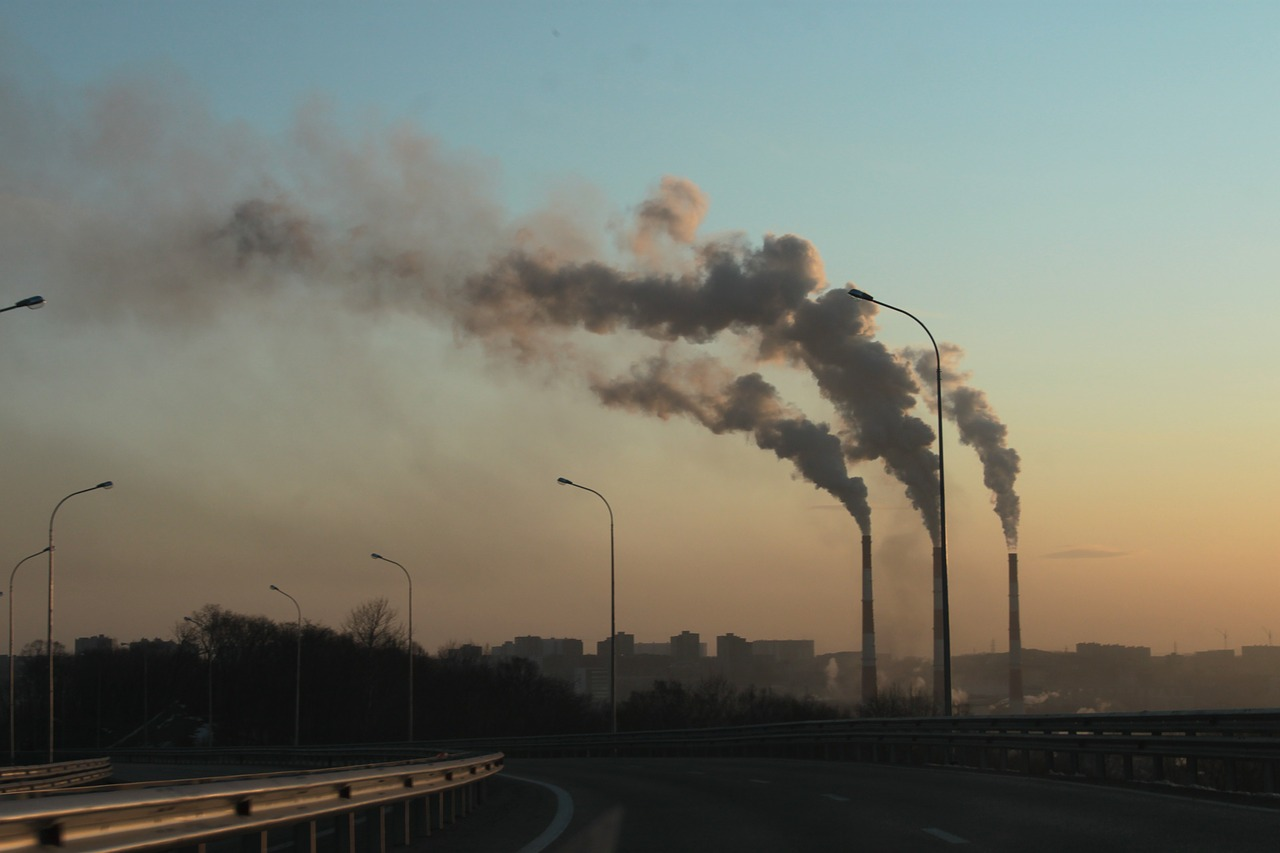
\includegraphics[scale=0.08]{Factory1}}
The twist in this problem is that the growth rate is not explicitly given, so we'll have to find it before we can make our prediction.

We will let 1990 correspond to year 0, so 2000 is year 10.
\begin{center}
\begin{tabular}{c c}
\textbf{Year} & \textbf{Emissions (million tons)}\\
\hline
0 & 962\\
10 & 1182
\end{tabular}
\end{center}
We can put this information into the exponential growth model:
\begin{align*}
P_{10} &= P_0(1+r)^{10}\\
1182 &= 962(1+r)^{10}
\end{align*}

Now we need to solve for $r$:
\begin{center}
\begin{tabular}{c l}
$1182 = 962(1+r)^{10}$ & Divide both sides by 962\\
& \\
$\dfrac{1182}{962} = (1+r)^{10}$ & Take the 10th root of both sides\\
& \\
$\sqrt[10]{\dfrac{1182}{962}} = 1+r$ & Subtract 1 from both sides\\
& \\
$\sqrt[10]{\dfrac{1182}{962}}-1 = r$ &
\end{tabular}
\end{center}
\[r=\sqrt[10]{\dfrac{1182}{962}}-1 = 0.0208 = 2.08\%\]

So if the emissions are growing exponentially, they are growing by about 2.08\% per year.  We can use this to predict the emissions in 2050, using 1990 as year 0:
\[P_{60} = 962(1+0.0208)^{60} = 2208.4 \textrm{ million metric tons of CO}_2 \textrm{ in 2050}\]
\end{example}

\begin{try}[http://www.izzomath.com/103text/growthmodels/example2.3/story.html]
The number of users on a social networking site was 45,000 in February when they officially went public, and grew to 60,000 by October.  If the site is growing exponentially and growth continues at the same rate, how many users should they expect two years after they went public?
\end{try}

\begin{proc}{Using Your Calculator: Roots}
In the previous example, we had to calculate the 10th root of a number.  Many scientific calculators have a button for general roots that looks like:
\begin{center}
\begin{tabular}{c c c}
$\boxed{\sqrt[n]{\hspace{0.1in}}}$ & $\boxed{\sqrt[x]{\hspace{0.1in}}}$ & $\boxed{\sqrt[y]{x}}$
\end{tabular}
\end{center}

To evaluate the 3rd root of 8, for example, we'd type either 3 $\boxed{\sqrt[n]{\hspace{0.1in}}}$ 8 or 8 $\boxed{\sqrt[n]{\hspace{0.1in}}}$ 3, depending on the calculator.  Try it on yours to see---you should get 2.\\

If you can't find a general root button, you can use the property of exponents that \[\sqrt[n]{a} = a^{1/n}.\]
To compute $\sqrt[3]{8}$, then, you could use the exponent key on your calculator to evaluate $8^{1/3}$.  Make sure that you use parentheses to preserve order of operations:
\[8\ \boxed{y^x}\ (\ 1\ \boxed{\div}\ 3\ )\]
\end{proc}

\paragraph{Rounding} If we had rounded the growth rate to 2.1\%, our calculation for the emissions in 2050 would have been 3347.  Rounding to 2\% would have given a result of 3156.  A very small difference in the growth rate gets magnified greatly in exponential growth.  Thus, round the growth rate as little as possible, keeping at least three significant digits (numbers after any leading zeros).  For instance, 0.41624 could be reasonably rounded to 0.416, and a growth rate of 0.001027 could be rounded to 0.00103.

\paragraph{Is the data linear or exponential?} So far in these examples, we've been told whether to use a linear model or an exponential one to make predictions, but the real world is not so accommodating; we often need to determine which kind of model we want to use.  To determine what kind of model will produce the best results, we can do a couple of things:
\begin{enumerate}
\item Plot data values from the past, as many as you can.  Look for a trend; does the data appear to be following a line, or does the curve look more like an exponential graph?  Keep in mind that in the short term, the difference is not that dramatic.
\item Think about the actual factors at play in the scenario; are they things you would expect to change linearly or exponentially?  For example, in the case of carbon emissions, we could expect that they might be tied closely to population values, which tend to change exponentially, since population growth is a percentage of the current population.
\end{enumerate}

\subsection{Exponential Growth with $e$}
What makes exponential growth exponential?  For instance, $1.005^t$ is exponential but $t^{1.005}$ is not, although there is an exponent in both.  The difference lies in where the variable $t$ is located---this is the quantity that varies in the model, and the one for which we want to predict results.  If the variable is in the \textit{base} of the exponent, it is not an exponential model, but only if the variable is in the \textit{exponent}.

We've seen several exponential models with different bases, but there is one base that is used more than any other: the natural base.\footnote{See the section on continuously compounded interest in the Financial Math chapter for more information.}  This is an irrational number (meaning it cannot be written as a fraction and its decimal form has digits after the decimal point that go on without end), and the letter $e$ is reserved for it: \[e = 2.71828 \ldots\]
It turns out that any exponential model, no matter the base, can be rewritten using the natural base, so if you encounter exponential models elsewhere, they may all be written with $e$ as the base.
\pagebreak

\begin{example}[https://www.youtube.com/watch?v=w8k-ob4i2U0]{US Population}
The population in the United States has been growing approximately according to the following exponential model since 1930:
\[P_t = 123.1e^{0.01217t}\]
where population is measured in millions.

Interpret this model and use it to predict the population in 2000.\\

\marginnote{\includegraphics[scale=0.1]{USPop1}}
If we let $t=0$ (1930), notice that $e^{(0.01217)(0)} = 1$ (remember, anything raised to 0 equals 1), so $P_0 = 123.1$.  Thus, we conclude that the population was 123.1 million in 1930, and the growth rate is 1.217\% (although growth rate means something slightly different than it did before we introduced $e$).\\

To predict the population in 2000, simply let $t=70$:
\[P_{70} = 123.1e^{(0.01217)(70)} = 288.5\]
This model predicts that the 2000 US population would be 288.5 million people, while the actual population in 2000 was 282.2 million.  Again, the model isn't perfect, but considering that we used it to predict a value 70 years in the future, it ended up performing pretty well.  Remember, the further we extrapolate, the worse our results will be.
\end{example}

\begin{try}[http://www.izzomath.com/103text/growthmodels/example2.4/story.html]
A colony of bacteria is growing exponentially according to the following model:
\[P_t = 1200e^{0.035t}\]
where $t$ is measured in weeks.
\begin{enumerate}
\item What was the initial population?
\item Use this model to predict the population after 7 weeks.
\end{enumerate}
\end{try}

\subsection{Radioactive Decay}
So far, all of the examples have featured exponential \textit{growth}, meaning that the values increased over time.  However, there are times where we may study quantities that \textit{decrease} over time according to an exponential model.  We'll use the natural base for the exponential models here.

In an exponential model like
\[P_t = P_0 e^{kt}\]
$k$ is called the growth rate.  As $t$ gets larger, $e^{kt}$ gets larger as well, and the quantity grows.  However, if we want to talk about exponential \textit{decay}, where the quantity is decreasing, what should we change?

Since $k$ is called the growth rate, we might think to start there.  In all of the examples we've seen so far, $k$ has been positive.  What if we make it negative?  To ask that another way, what happens when we raise $e$ to a negative number?  Do we get a negative result?

It may help to remember an exponent rule: $x^{-a} = \dfrac{1}{x^a}$

Thus,
\begin{align*}
e^{-1} &= \dfrac{1}{e^1} \approx 0.368\\
e^{-2} &= \dfrac{1}{e^2} \approx 0.135\\
e^{-3} &= \dfrac{1}{e^3} \approx 0.050\\
e^{-4} &= \dfrac{1}{e^4} \approx 0.018\\
\end{align*}
and you begin to see the trend.  If $k$ is negative, the exponent will be negative, making $e^{kt}$ smaller as $t$ increases, meaning that the total quantity $P_t$ will decrease as $t$ increases.  This is exponential decay.

\begin{formula}{Exponential Growth and Decay}
\marginnote{\footnotesize Note that although $k$ is also called a growth rate, it belongs to a different model than the earlier growth rate $r$}
Consider a general exponential model
\[P_t = P_0 \ e^{kt}\]

If $k$ is positive, it is called the \textbf{growth rate}, and $P_t$ increases as $t$ increases.

If $k$ is negative, it is called the \textbf{decay rate}, and $P_t$ decreases as $t$ increases.
\end{formula}

\begin{example}[https://www.youtube.com/watch?v=6SIiItzYfQo]{Radioactive Decay}
Radioactive gold 198, used in imaging the structure of the liver, decays exponentially according to the following model:
\[A_t = A_0 \ e^{-0.2596t}\] where $t$ is measured in days.  If we start with 50 milligrams of the isotope, how many milligrams will be left after a week?\\

\marginnote{\bfseries Solution}
Simply let $t=7$:
\[A_7 = 50e^{-0.2596(7)} = 8.12 \textrm{ milligrams}\]
As expected, there is less after a week than we started with.
\end{example}

\begin{try}[http://www.izzomath.com/103text/growthmodels/example2.5/story.html]
The atmospheric pressure $p$ on a plane decreases with increasing height.  This pressure, measured in mmHg, is related to the height $h$ in km above sea level by the model $p=760e^{-0.145h}$  Find the atmospheric pressure at a height of 2 km above sea level.
\end{try}

\subsection{Using Logarithms to Solve for Time}
At the beginning of this section, we modeled the population growth of Frederick County from 2013 onward using the following equation:
\vspace{0.1in}
\[P_t = 241,409(1+0.008)^t\]
\vspace{0.1in}

We can use this equation to predict the population at any point in the future (albeit imperfectly) if we have a year that we're interested in.  What if we flip the problem around, though?  What if, instead of being given a year and asked to find the population, we were interested in knowing what year the population hit a certain mark? \\ 

For instance, what if we wanted to know when the population of Frederick County would reach 400,000?  Here $P_t$ is given and $t$ is what we're looking for:
\vspace{0.1in}

\begin{center}
\begin{tabular}{r @{ $=$ } l l}
400,000 & $241,409(1.008)^t$ & Divide both sides by 241,409\\
1.657 & $1.008^t$ & We need to solve this for $t$
\end{tabular}
\end{center}
\vfill
\pagebreak

One way to make this prediction would be to create a table of values, or draw a graph using a computer or graphing calculator.
\begin{center}
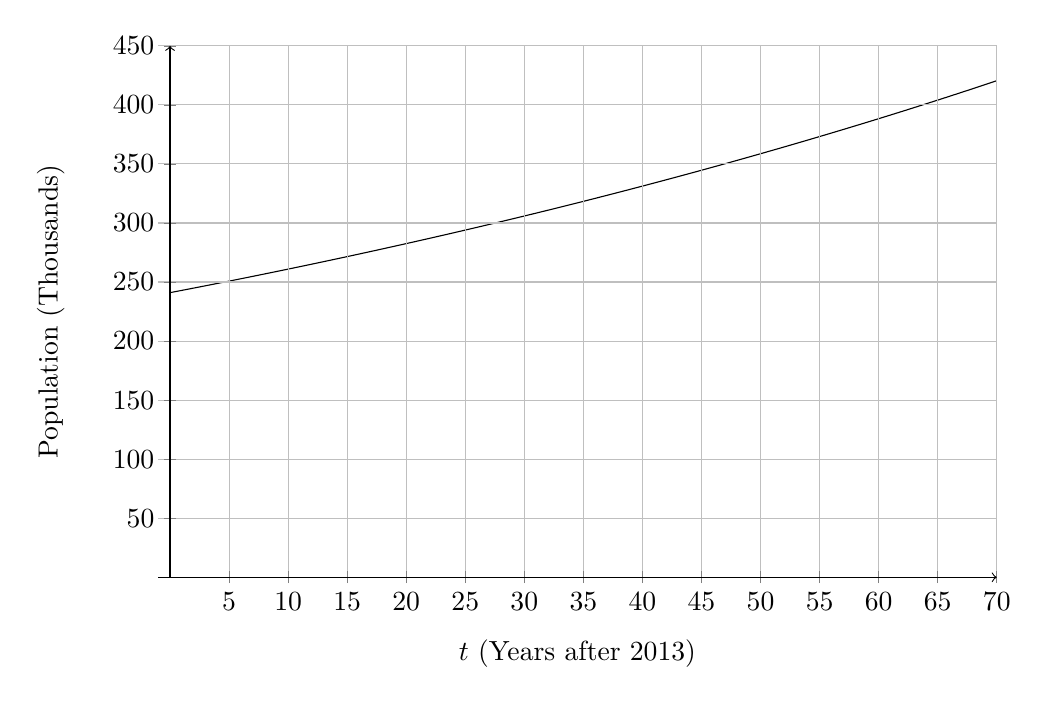
\begin{tikzpicture}
\begin{axis}[
    xmin=-1, xmax=70,
    ymin=0, ymax=450,
    axis lines=center,
    axis on top=true,
    domain=0:1,
    x=0.15cm,
    y=0.015cm,
    xtick={0,5,...,100},
    xticklabels={0,5,...,100},
    ytick={0,50,...,450},
    yticklabels={0,50,...,450},
    axis lines=middle,
    axis line style={->},
    x label style={at={(axis description cs:0.5,-0.1)},anchor=north},
    y label style={at={(axis description cs:-0.1,.5)},rotate=90,anchor=south},
    xlabel={$t$ (Years after 2013)},
    ylabel={Population (Thousands)},
    grid=major
    ]
	\addplot[samples=100,domain=0:70] {241*(1.008^x)};
\end{axis}
\end{tikzpicture}
\end{center}

From the graph, we can estimate that the population will reach 400,000 somewhere between 60 and 65 years after 2013 (2073 to 2078), but we can do better than this.  To get a more precise answer, we turn to an algebraic tool known as the \textbf{logarithm}.

Today\footnote{Before computers were ubiquitous, logarithms were used to make hand calculations easier, especially useful when creating huge tables of navigational data}, one of the two main uses of logarithms is to solve equations like this one where the unknown lies in the exponent.  Just like a square root undoes a square, freeing the variable:
\[x^2 \longrightarrow \sqrt{x^2} = x\]
a logarithm undoes an exponential, freeing the variable from the exponent:
\[10^x \longrightarrow \log_{10} (10^x) = x\]

Each base has a logarithm to go with it, so to isolate the variable in $3^x$, we'd use $\log_3$, for $7^x$ we'd use $\log_7$, and so on.  We'll focus on two in particular, though: $\log_{10}$, which is abbreviated $\log$, and $\log_e$, which is abbreviated $\ln$ (meaning natural log)\footnote{From the Latin \textit{logarithmus naturalis}}.  These are the two that are easily accessible on most calculators, and all other logarithms can be calculated using either of these two.

\begin{formula}{The Common and Natural Logarithm}
The \textbf{common logarithm}, written $\log (x)$, undoes the exponential $10^x$:
\[\log(10^x) = x \textrm{ and } 10^{\log(x)} = x\]

The \textbf{natural logarithm}, written $\ln (x)$, undoes the exponential $e^x$:
\[\ln(e^x) = x \textrm{ and } e^{\ln(x)} = x\]

Any other logarithm can be written in terms of either of these by using the \textbf{change of base formula}:
\[\log_b(x) = \dfrac{\log(x)}{\log(b)} \textrm{ or } \log_b(x) = \dfrac{\ln(x)}{\ln(b)}\]
\end{formula}
\pagebreak

Before we begin using logarithms to solve equations like the one in the population example, let's get some practice with them.

\begin{example}[https://www.youtube.com/watch?v=_OTEHIGS3qM]{Common Logarithm}
Evaluate each of the following:
\begin{center}
\begin{tabular}{l l l l l}
(a) $\log(100)$ & (b) $\log(1000)$ & (c) $\log(10,000)$ & (d) $\log\left(\dfrac{1}{100}\right)$ & (e) $\log(1)$
\end{tabular}
\end{center}

\marginnote{\bfseries Solution}
\begin{enumerate}[(a)]
\item $\log(100)$ can be written as $\log\left(10^2\right) = 2$
\item $\log(1000) = \log\left(10^3\right) = 3$
\item $\log(10,000) = \log\left(10^4\right) = 4$
\item Recall that $x^{-n} = \dfrac{1}{x^n}$, so $\log\left(\dfrac{1}{100}\right) = \log\left(10^{-2}\right) = -2$
\item Recall that $x^0=1$, so $\log(1) = \log\left(10^0\right) = 0$
\end{enumerate}
\end{example}

\begin{try}[http://www.izzomath.com/103text/growthmodels/example2.6/story.html]
Evaluate each of the following:
\begin{center}
\begin{tabular}{l l l l l}
(a) $\ln(e)$ & (b) $\ln(e^2)$ & (d) $\ln\left(\dfrac{1}{e^3}\right)$ & (e) $\ln(1)$
\end{tabular}
\end{center}
\end{try}

What if the number we're trying to evaluate with a logarithm can't be written as a power of 10 or $e$?  For this, our calculator comes to the rescue.

\begin{proc}{Using Your Calculator: Logarithms}
\begin{center}
\begin{tabular}{l b{3in}}
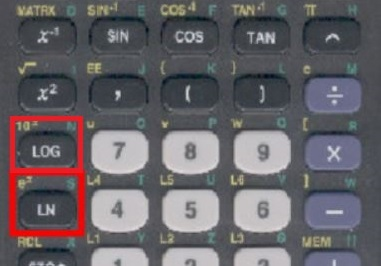
\includegraphics[scale=0.3]{CalculatorLog} & Look for buttons labeled LOG and LN on your calculator.  Try the answers in the example above to check yourself.
\end{tabular}
\end{center}
\end{proc}

\begin{example}[https://www.youtube.com/watch?v=AE02zNX0nVg]{Evaluating Logarithms with a Calculator}
Evaluate each of the following with a calculator:
\begin{center}
\begin{tabular}{l l l l}
(a) $\log(300)$ & (b) $\log(4.5)$ & (c) $\ln(31)$ & (d) $\ln(0.1)$\\
\marginnote{\bfseries Solution}
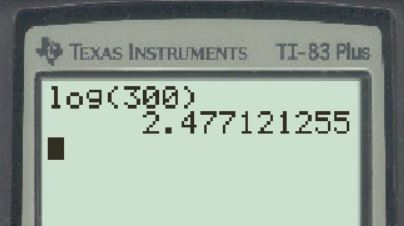
\includegraphics[height=0.6in]{CalculatorLog300} & 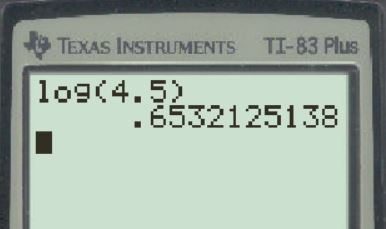
\includegraphics[height=0.6in]{CalculatorLog45} & 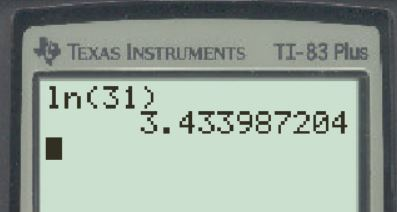
\includegraphics[height=0.6in]{CalculatorLn31} & 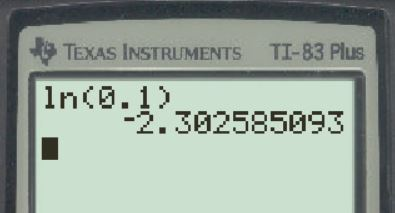
\includegraphics[height=0.6in]{CalculatorLn01}\\
2.477 & 0.653 & 3.434 & $-2.303$
\end{tabular}
\end{center}
\end{example}

\begin{try}[http://www.izzomath.com/103text/growthmodels/example2.7/story.html]
Evaluate each of the following with a calculator:
\begin{center}
\begin{tabular}{l l l l}
(a) $\log(0.5)$ & (b) $\log(27)$ & (c) $\ln(2)$ & (d) $\ln(0.85)$
\end{tabular}
\end{center}
\end{try}
\pagebreak

What about something like $\log_5(30)$?  Can we use our calculator to evaluate this?  Some calculators have a function for logarithms with any base, but if they do, it's buried in a menu somewhere.  Instead, we'll use the change-of-base formula, since that only requires using either the LOG key or the LN key, which most calculators have.
\[\log_5(30) = \dfrac{\log(30}{\log(5)} = \dfrac{1.477}{0.699} = 2.113\]

Notice that if we used the change-of-base formula with LN instead, we'd get the same answer:
\[\log_5(30) = \dfrac{\ln(30}{\ln(5)} = \dfrac{3.401}{1.609} = 2.113\]

Thus, you can use the change-of-base formula with either LOG or LN to evaluate logarithms with any base.

\begin{try}
Evaluate each of the following with a calculator:
\begin{center}
\begin{tabular}{l l l l}
(a) $\log_3(12)$ & (b) $\log_{1.5}(99)$ & (c) $\log_{0.7}(3)$ & (d) $\log_{23}(1.77)$
\end{tabular}
\end{center}
\end{try}

Now we finally get to the point of this: solving exponential equations using logarithms.  Remember that the key to solving equations in general is that whatever we do to one side, we must do to the other.  Just like we can add anything to both sides or square both sides, we can also take the logarithm of both sides of an equation and end up with an equivalent equation.  Since logarithms undo exponentials, this will simplify an equation that has a variable in the exponent.

\begin{example}[https://www.youtube.com/watch?v=JnA4ypiJB6g]{Solving Equations with Logarithms}
Solve each of the following equations:
\begin{center}
\begin{tabular}{l l l l}
(a) $10^x=1000$ & (b) $10^x=3$ & (c) $2(10^x)=8$ & (d) $e^x=5$\\
(e) $3e^x=12$ & (f) $2.5^x=17$ & (g) $0.2^x=2$ & (h) $50(1.04^x)=125$
\end{tabular}
\end{center}

\marginnote{\bfseries Solution}
\begin{enumerate}[(a)]
\item Take the log of both sides: \[\log(10^x) = \log(10^3) \longrightarrow x=3\]
\item Take the log of both sides: \[\log(10^x) = \log(3) \longrightarrow x=\log(3) \approx 0.477\]
\item Isolate the exponential before taking the log of both sides:
\[2(10^x)=8 \longrightarrow 10^x = 4 \longrightarrow x=\log(4) \approx 0.602\]
\item Use the natural log this time:
\[e^x=5 \longrightarrow \ln(e^x) = \ln(5) \longrightarrow x=\ln(5) \approx 1.609\]
\item Again, isolate the exponential, and use the natural log:
\[3e^x = 12 \longrightarrow e^x=4 \longrightarrow x=\ln(4) \approx 1.386\]
\item Here we have to use the change-of-base formula:
\[2.5^x=17 \longrightarrow \log_{2.5}(2.5^x)=\log_{2.5}(17) \longrightarrow x = \dfrac{\log(17)}{\log(2.5)} \approx 3.092\]
\item Again, using the change-of-base formula:
\[0.2^x = 2 \longrightarrow x=\log_{0.2}(2) = \dfrac{\log(2)}{\log(0.2)} \approx -0.4307\]
\item Isolate the exponential before using the change-of-base formula:
\[50(1.04^x) = 125 \longrightarrow 1.04^x = 2.5 \longrightarrow x = \log_{1.04}(2.5) = \dfrac{\log(2.5)}{\log(1.04)} \approx 23.36\]
\end{enumerate}
\end{example}
\pagebreak

\begin{try}[http://www.izzomath.com/103text/growthmodels/example2.8/story.html]
Solve each of the following equations:
\begin{center}
\begin{tabular}{l l l l}
(a) $10^x=4$ & (b) $5e^x=8$ & (c) $2^x=75$ & (d) $20(1.95^x)=140$
\end{tabular}
\end{center}
\end{try}

Now that we can use logarithms to solve exponential equations with any base, we can return to our discussion of the population model for Frederick County.  Recall that we have the model
\[P_t = 241,409(1.008^t)\]
and we asked when the population would reach 400,000, which led to the equation \[1.657=1.008^t\] where we want to solve for $t$.  Now we know how to do this:
\[1.008^t=1.657 \longrightarrow t = \log_{1.008} (1.657) = \dfrac{\log(1.657)}{\log(1.008)} \approx 63.4\]
We conclude that according to this model, the population of Frederick County will reach 400,000 about 63 years after 2013, or the year 2076.

\begin{example}[https://www.youtube.com/watch?v=ei5RaBwgRNc]{Filtering Water}
Polluted water is passed through a series of filters.  Each filter removes 90\% of the remaining impurities from the water.  If you have 10 million particles of pollutant per gallon originally, how many filters would the water need to be passed through to reduce the pollutant to 500 particles per gallon?\\

\marginnote{\includegraphics[scale=0.15]{ROFilter}\\\footnotesize\textcolor{black!60}{From Wikipedia}\\\footnotesize\textcolor{black!60}{Photo by Twhair}}
In this problem, our ``population'' is the number of particles of pollutant per gallon.  The initial pollutant is 10 million particles per gallon, so \[P_0 = 10,000,000.\]  Instead of changing with time, the population changes with the number of filters, so $t$ will represent the number of filters used.

Since the amount of pollutant is decreasing with each filter, this is an example of exponential decay, with a decay rate of $r=-0.90$.

The decay model is
\[P_t = 10,000,000(1-0.90)^t = 10,000,000(0.1^t).\]

To answer the question of how many filters are needed to lower the pollutant to 500 particles per gallon, we set $P_t$ to 500 and solve for $t$:
\begin{center}
\begin{tabular}{r @{ $=$} l l}
500 & $10,000,000(0.1^t)$ & Divide both sides by 10,000,000\\
0.00005 & $0.1^t$ & Take the $\log_{0.1}$ of both sides\\
$\log_{0.1}(0.00005)$ & $t$ & Use the change-of-base formula\\
$\dfrac{\log(0.00005)}{\log(0.1)}$ & $t$ & Approximate with a calculator\\
4.301 & $t$
\end{tabular}
\end{center}
It would take about 4.301 filters to reduce the pollutant to the desired level, but since we can't install 0.3 filters, we would need to use 5 filters to reach the goal.
\end{example}

\begin{try}[http://www.izzomath.com/103text/growthmodels/example2.9/story.html]
India had a population in 2008 of about 1.14 billion people, growing by about 1.34\% each year.  If this trend continued, when was India's population expected to reach 1.2 billion?
\end{try}
\vfill
\pagebreak

\subsection{Application: Newton's Law of Cooling}
If you leave a hot cup of coffee out on the counter, you expect it to cool over time as it loses heat to the environment, or the \textit{medium}.  The rate at which this heat transfer occurs depends on many things, like the composition of the fluid, the humidity of the air, the materials of the coffee cup and the counter, and so on.  However, the most significant factor that controls this rate is the difference in temperature between the coffee cup and the environment; when the coffee is much hotter than the air around it, it will cool much more rapidly than when its temperature is closer to that of the air.  Over time, the coffee will approach room temperature and the transfer of heat will slow down.  Specifically, the temperature will decrease according to the equation \[T=T_m+(T_0-T_m)e^{kt}\] where $T$ is the temperature of the object (changing over time), $T_m$ is the temperature of the medium (the surroundings), $T_0$ is the initial temperature of the object (e.g. the coffee cup), and $k$ is the decay rate--a negative constant that depends on all of those other factors related to the environment and the materials.  This model also works if the object is cooler than the environment and warming over time, like if you placed a cup of ice water on the counter instead.\\

For example, suppose a coffee cup at 180$^{\circ}$ F is allowed to cool in a room whose air temperature is 65$^{\circ}$ F.
\begin{enumerate}
\item If the temperature of the cup is 120$^{\circ}$ F after 10 minutes, what is $k$?\\

Plug the given information into the equation and use logarithms to solve for $k$:
\begin{align*}
T &= T_m+(T_0-T_m)e^{kt}\\
120 &= 65 + (180-65)e^{k(10)}\\
55 &= 115e^{10k}\\
0.478 &= e^{10k}\\
\ln(0.478) &= 10k\\
-0.7376 &= 10k\\
-0.0738 &= k
\end{align*}

\item What will its temperature be after 20 minutes?\\

Let $t=20$ in the model, since now we know $k$:
\[T=65+(180-65)e^{-0.0738(20)} = 91.3\]
Thus we expect it to reach about 91$^{\circ}$ F after 20 minutes.

\item When will it reach 80$^{\circ}$ F?\\

Let $T=80$ and solve for $t$ using a logarithm:
\begin{align*}
80 &= 65+115e^{-0.0738t}\\
15 &= 115e^{-0.0738t}\\
0.1304 &= e^{-0.0738t}\\ 
-0.0738t &= \ln(0.1304)\\ 
t &\approx 27.6
\end{align*}
We expect the coffee cup to reach 80$^{\circ}$ F after about 28 minutes.
\pagebreak

\item Graph the temperature over time.
\begin{center}
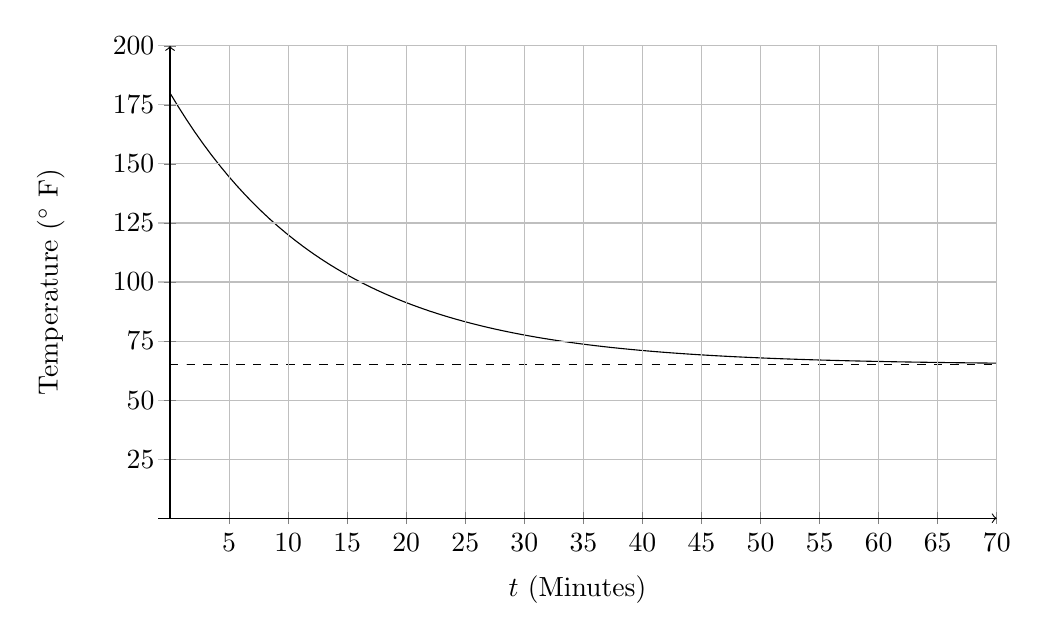
\begin{tikzpicture}
\begin{axis}[
    xmin=-1, xmax=70,
    ymin=0, ymax=200,
    axis lines=center,
    axis on top=true,
    domain=0:1,
    x=0.15cm,
    y=0.03cm,
    xtick={0,5,...,100},
    xticklabels={0,5,...,100},
    ytick={0,25,...,200},
    yticklabels={0,25,...,200},
    axis lines=middle,
    axis line style={->},
    x label style={at={(axis description cs:0.5,-0.1)},anchor=north},
    y label style={at={(axis description cs:-0.1,.5)},rotate=90,anchor=south},
    xlabel={$t$ (Minutes)},
    ylabel={Temperature ($^{\circ}$ F)},
    grid=major
    ]
	\addplot[samples=100,domain=0:70] {65+115*e^(-0.0738*x)};
	\addplot[samples=100,domain=0:70,dashed] {65};
\end{axis}
\end{tikzpicture}
\end{center}

Notice the exponential shape of the curve, and notice that it predicts what we expected, that the temperature approaches 65$^{\circ}$ F over time; we call that behavior \textit{asymptotic}, since as $t$ gets larger, the temperature approaches 65 but never crosses below that.  As we noted, the rate of decrease is much larger at first, when the temperature difference is large, but it slows as the coffee's temperature gets closer to the room temperature.
\end{enumerate}

\begin{exercises}
\textit{In Exercises 1---8, evaluate each logarithm.}

\pfour{$\log(10)$}
\pfour{$\ln(e)$}
\pfour{$\log(23)$}
\pfour{$\ln(50)$}

\pfour{$\log\left(\dfrac{1}{1000}\right)$}
\pfour{$\ln\left(\dfrac{1}{e^5}\right)$}
\pfour{$\log_{1.5}(42)$}
\pfour{$\log_{0.57}(18)$}

\textit{In Exercises 9---16, solve each exponential equation.}

\pfour{$10^x=100$}
\pfour{$10^x=5$}
\pfour{$e^x=8$}
\pfour{$e^{2x}=19$}

\pfour{$4(10^x)=9$}
\pfour{$7^x=100$}
\pfour{$9(3^{2x})=56$}
\pfour{$22e^{0.05x}=37$}

\ptwo{Tacoma's population in 2000 was about 200 thousand, and had been growing by about 9\% per year.
\begin{enumerate}[(a)]
\item Write an explicit formula for the population of Tacoma.
\item If this trend continues, what will Tacoma's population be in 2016?
\item When does this model predict Tacoma's population to exceed 400 thousand?
\end{enumerate}}
\ptwo{Portland's population in 2007 was about 568 thousand, and had been growing by about 1.1\% per year.
\begin{enumerate}[(a)]
\item Write an explicit formula for the population of Portland.
\item If this trend continues, what will Portland's population be in 2016?
\item When does this model predict Portland's population to reach 700 thousand?
\end{enumerate}}

\ptwo{Diseases tend to spread exponentially.  In the early days of AIDS, the growth rate was around 190\%.  In 1983, about 1700 people in the US died of AIDS.  If the trend had continued unchecked, how many people would have died from AIDS in 2005?}
\ptwo{The population of the world in 1987 was 5 billion and the annual growth rate was estimated at 2 percent.  If the world population followed an exponential growth model, find the projected world population in 2015.}

\ptwo{A bacteria culture is started with 300 bacteria.  After 4 hours, the population has grown to 500 bacteria.  If the population grows exponentially according to the formula $P_t = P_0(1+r)^t$,
\begin{enumerate}[(a)]
\item Find the growth rate $r$ and write the full formula.
\item If this trend continues, how many bacteria will there be in one day?
\item How long will it take for this culture to triple in size?
\end{enumerate}}
\ptwo{A native wolf species has been reintroduced into a national forest.  Originally 200 wolves were transplanted, and after 3 years, the population had grown to 270 wolves.  If the population grows exponentially according to the formula $P_t = P_0(1+r)^t$,
\begin{enumerate}[(a)]
\item Find the growth rate $r$ and write the full formula.
\item If this trend continues, how many wolves will there be in ten years?
\item If this trend continues, how long will it take the population to grow to 1000 wolves?
\end{enumerate}}

\ptwo{The population in millions of the state of New Jersey has grown since 1973 according to the model $P_t=7.333e^{0.004t}$.
\begin{enumerate}[(a)]
\item What was the population of New Jersey in 1973?
\item What does this model predict the population of New Jersey would be in 1993?
\item According to this model, when will the population of New Jersey reach 9 million?
\end{enumerate}}
\ptwo{The population in millions of Colombia has grown since 1990 according to the model $P_t=33.31e^{0.018t}$.
\begin{enumerate}[(a)]
\item What was the population of Colombia in 1990?
\item What does this model predict the population of Colombia would be in 2000?
\item According to this model, when will the population of Colombia reach 52 million?
\end{enumerate}}

\ptwo{Strontium 90 is a radioactive isotope that decays according to the equation $A_t = A_0e^{-0.0244t}$, where $A_0$ is the initial amount present and $A_t$ is the amount present after $t$ years.  If you begin with 500 grams of strontium 90,
\begin{enumerate}[(a)]
\item How much strontium 90 will be left after 10 years?
\item When will 400 grams of strontium 90 be left?
\end{enumerate}}
\ptwo{Thorium 234 is a radioactive isotope that decays according to the equation $A_t = A_0e^{-10.498t}$, where $A_0$ is the initial amount present and $A_t$ is the amount present after $t$ years.  If you begin with 1000 grams of thorium 234,
\begin{enumerate}[(a)]
\item How much thorium 234 will be left after 0.5 years?
\item When will 250 grams of thorium 234 be left?
\end{enumerate}}

\ptwo{A hot bar of iron at 1,100$^{\circ}$ F is quenched in oil at 350$^{\circ}$ F.  After 2 minutes, the temperature of the iron is 750$^{\circ}$ F.
\begin{enumerate}[(a)]
\item Find the value for $k$ in Newton's Law of Cooling.
\item What will the temperature of the iron be after 10 minutes?
\item How long will it take for the iron to reach 400$^{\circ}$ F?
\end{enumerate}}
\ptwo{A frozen hot dog at $-32^{\circ}$ F is placed in a room at 70$^{\circ}$ F.  After 15 minutes, the temperature of the hot dog is 30$^{\circ}$ F.
\begin{enumerate}[(a)]
\item Find the value for $k$ in Newton's Law of Cooling.
\item What will the temperature of the hot dog be after 45 minutes?
\item How long will it take for the hot dog to reach 60$^{\circ}$ F?
\end{enumerate}}

\end{exercises}
